LZ is a second generation Dark Matter direct detection experiment. The detector will operate in Sanford Underground Research Facility in South Dakota, USA \cite{SURF}. At the core of the LZ experiment there is a two-phase Time Projection Chamber (TPC) containing seven fully active tonnes of liquid Xenon (LXe). The TPC is enclosed by a Xenon Skin, acrylic tanks filled with liquid scintillator and an water tank housing 120 PMTs. The detector will be located in the existing 250-ton water tank used by LUX. LZ will use a total liquid xenon mass of 10 tonnes, an active mass of 7 tonnes and a fiducial mass of 5.6 tonnes \cite{LZTDR}. Over a 3 year period of operation, the experiment will probe WIMP-nucleon cross sections down to $2 \times 10^{-48} cm^2$ at 100 GeV \cite{LZIntro}. A drawing of the LZ detector can be seen in Figure \ref{fig:LZDetector}. 
\begin{figure}[h]
\centering
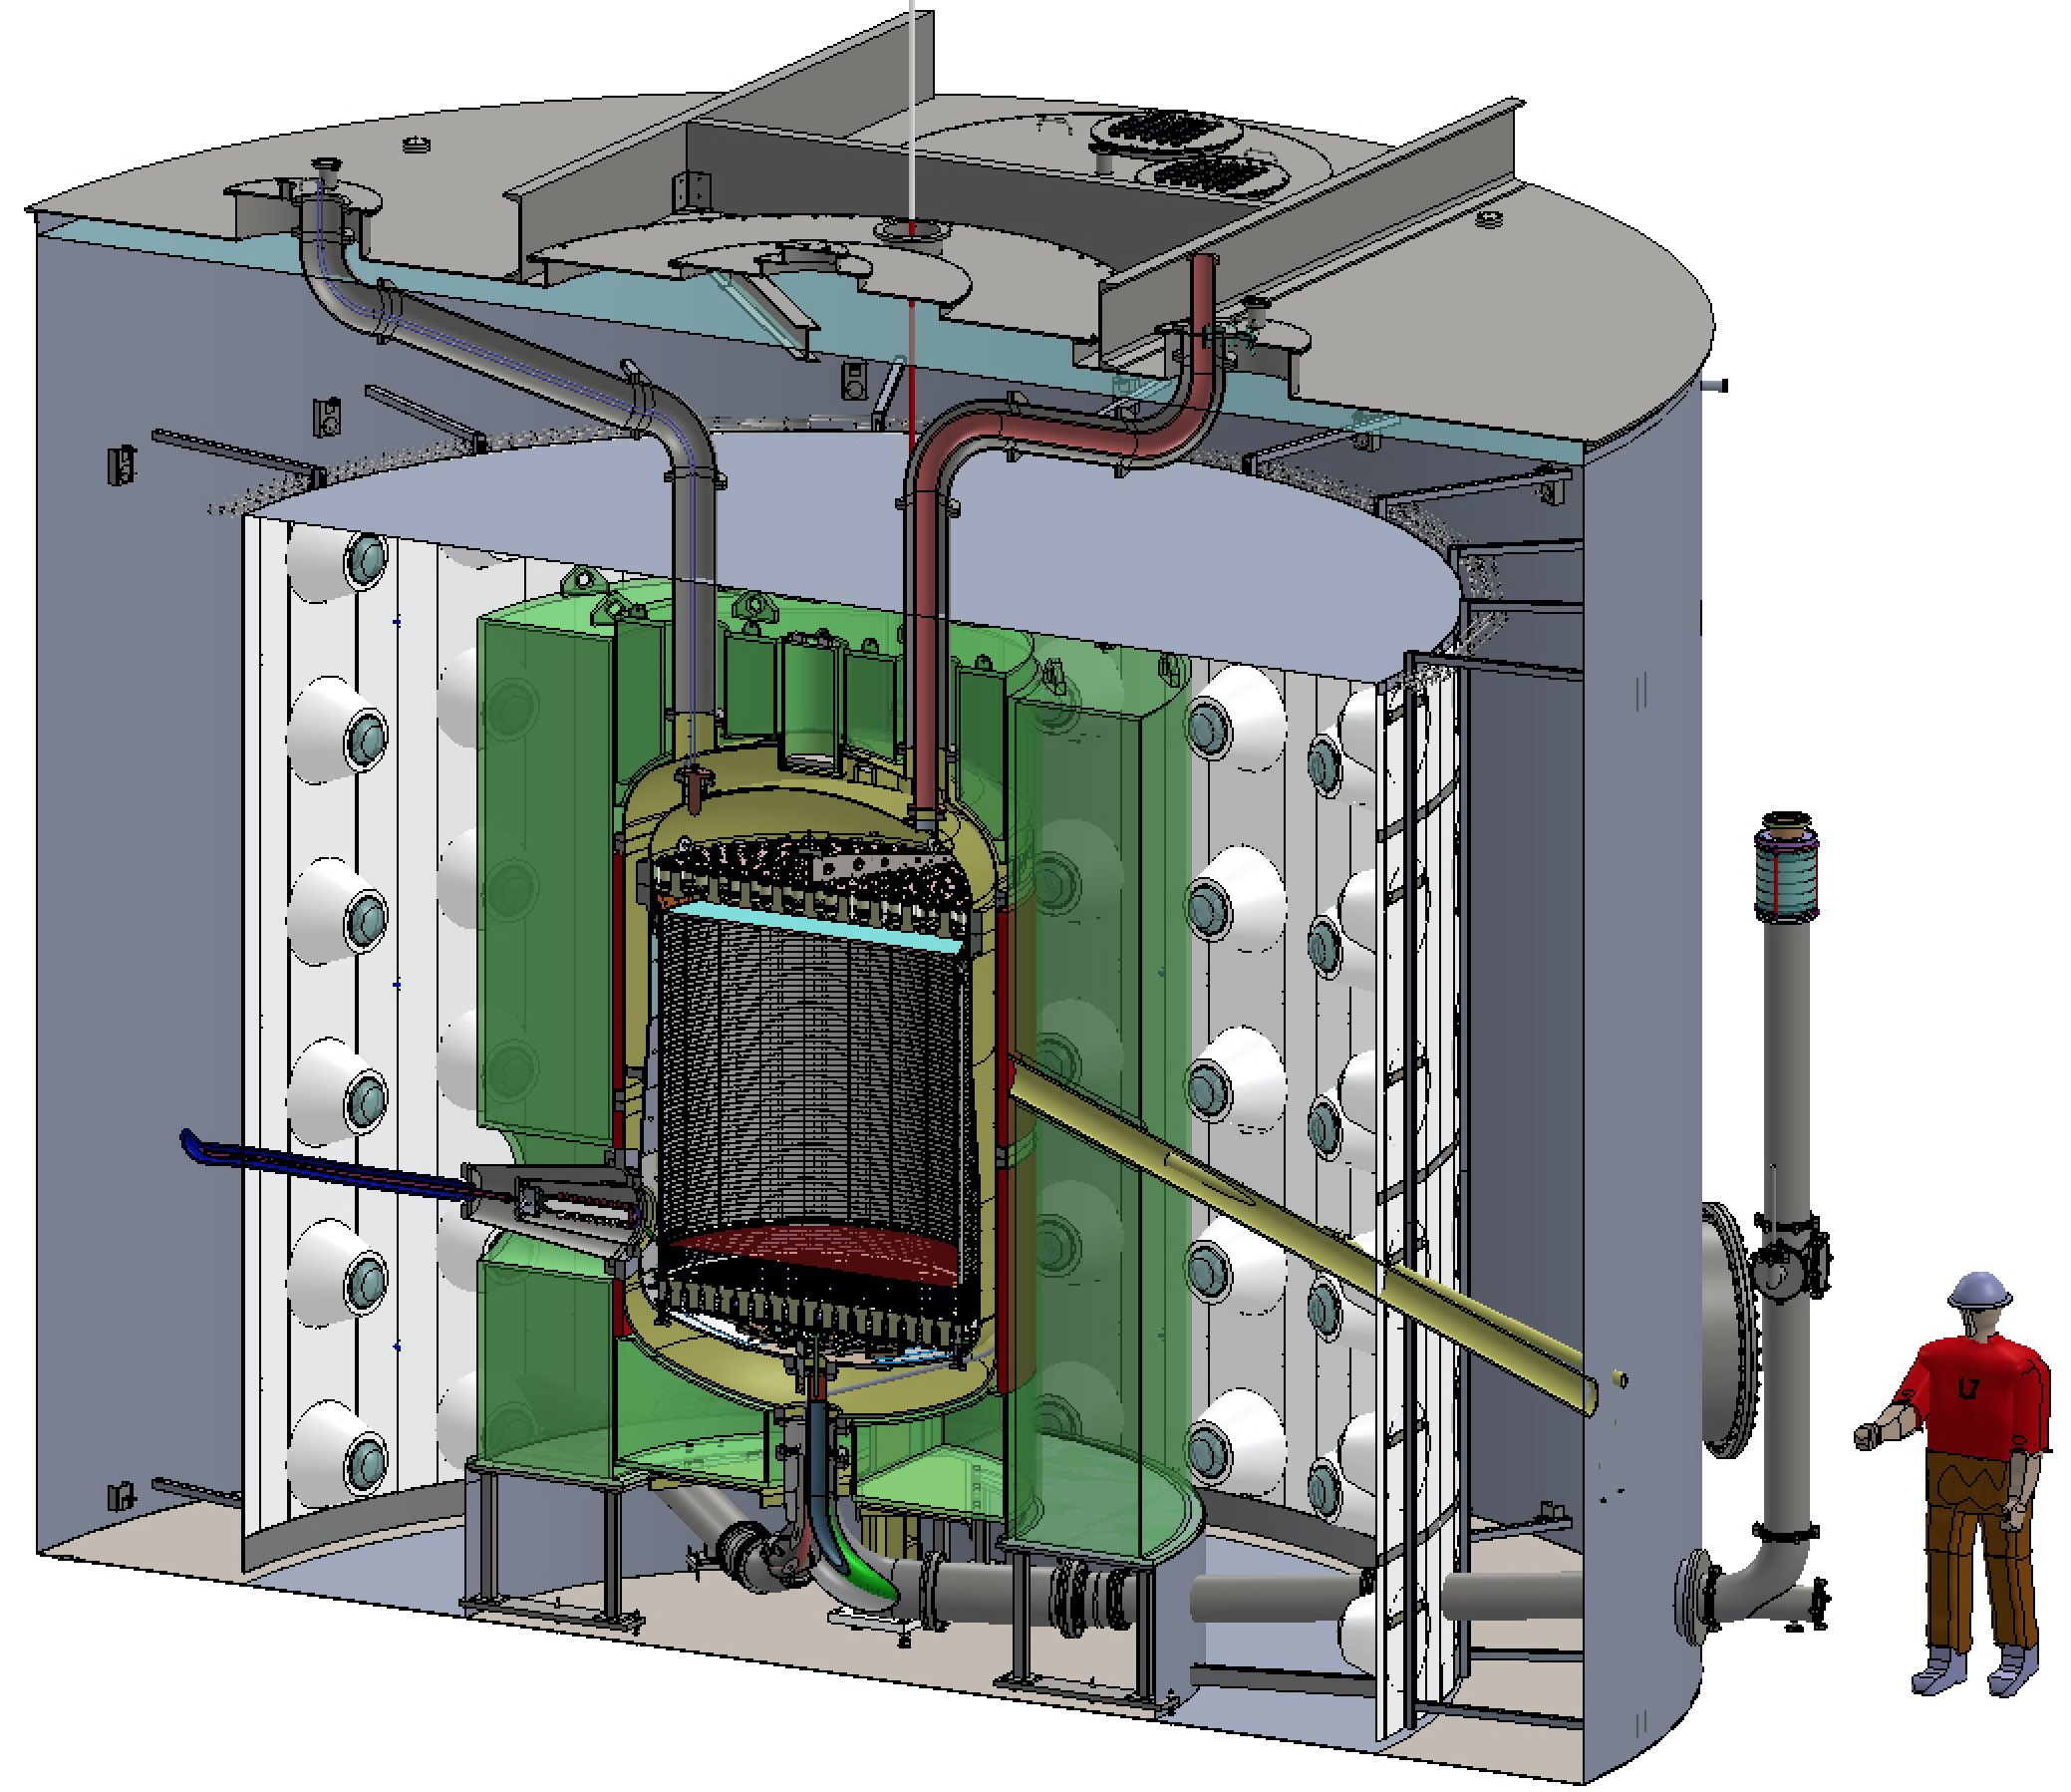
\includegraphics[width=0.7\textwidth]{Figures/Detector_design.jpg}
\caption{Cutaway drawing of the LZ detector systems. The LXe TPC is surrounded by the xenon skin layer (yellow), the scintillator tanks (green) and light collection system (white), all housed in a large water tank (blue-grey).\cite{LZTDR}}
\label{fig:LZDetector}
\end{figure}

\section{Dual phase LXe TPC}\label{sec:TPC}
As mention previously, the experiment will use a LXe TPC to detect a WIMP. After a WIMP interacts with a LXe atom in the TPC two signals are generated. In this interaction prompt scintillation light (S1) is produced from a nuclear recoil, this recoil also causes the ionisation of neighbouring atoms which produces free elections. These free elections are drifted upwards through the TPC using an induced electric field to the surface of the LXe, the free electrons are extracted in a gaseous phase and accelerated to produce a second scintillation signal (S2). Two arrays of photomultiplier tubes (PMTs), 253 on the top and 241 on bottom of the TPC measure the signals \cite{LZTDR}. The difference in time between the S1 signal and S2 signal is used to calculate the z-position in which the interaction occurs, the x-y position is determined by distribution of the S2 signal in the upper array of PMTs. The ratio of S2/S1 signals can be used to discriminate between different background sources and WIMP particles. A schematic of detection mechanism in dual phase TPC can be seen in figure \ref{fig:TPC_mech}. 

\begin{figure}[h]
    \centering
    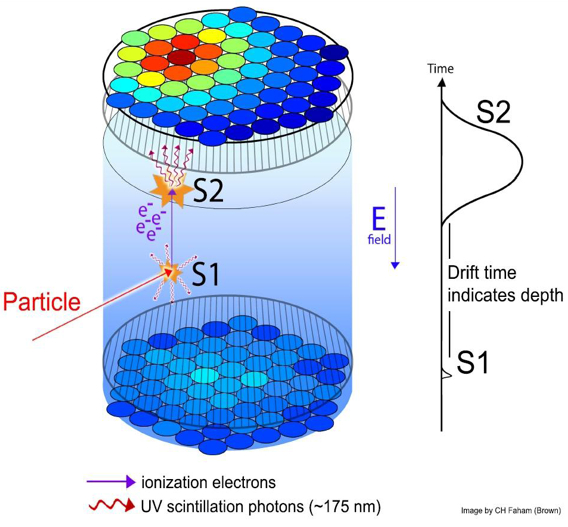
\includegraphics[width=0.6\textwidth]{Figures/TPC_mechanism.jpg}
    \caption{A schematic illustrating the principle in which a dual phase LXe TPC detects a WIMP interaction. When particle (WIMP) interacts with a LXe atom two signals are produced. The first signal produced is prompt scintillation light (S1) and the second signal produced are free electrons from the ionisation of neighbouring LXe atoms. The difference in time between S1 and S2 signal can be used to determine the z-position of the interaction and the distribution of light in the upper PMT array from the S2 signal can be used to determine the x-y position.  \cite{DMUCL}}
    \label{fig:TPC_mech}
\end{figure}

\section{Veto system}\label{sec:veto}
The TPC containing the large active volume of LXe is surrounded by a three-component veto system used to reject and characterise the background radiation from the surrounding environment. The first component of the veto system is the Xenon skin region located between the TPC and the cryostat walls, containing three tonnes of LXe, monitored by 131 PMTs. The second component of the veto system is ten acrylic tanks filled with seventeen tonnes of Gadolinium-loaded Liquid Scintillator (Gd-LS)\cite{LZTDR}.
The primary role of the scintillator is to tag neutrons which could cause nuclear recoils with a similar signature to that produced by WIMPs within the TPC. When the neutrons interact with the Gd-LS, scintillation light is produced and detected by an array of 120 8 inch Hamamatsu R5912 PMTs which surround the acrylic tanks. The third component of the veto system is ultra pure water surrounding the acrylic tanks. The ultra-pure water is used as a muon veto and shielding. The OD of LZ consists of the Gd-LS tanks, volume of water and is monitored by 120 PMT's
\newline
The layout of veto system can be seen in figure \ref{fig:LZDetector} where the Xenon skin layer is highlighted yellow, the Gd-LS Scintillator tanks in green and the PMT array mounted on a reflective screen of Tyvek\textregistered. An in depth description of the detector can be found in the LUX-ZEPLIN Technical Design Report (TDR) \cite{LZTDR}. In 2014, the University of Liverpool High Energy Particle group joined the LUX-ZEPLIN experiment. The group are responsible for the Optical Calibration System that will be used to calibrate the PMTs in the Outer Detector. This system will be discussed in chapter \ref{Chap6:OCS}. 